%======================================================================
%----------------------------------------------------------------------
%               XX                              X
%                                               X
%               XX    XXX   XXX   XXX      XXX  X  XXXX
%                X   X   X X   X X   X    X   X X X
%                X   XXXXX XXXXX XXXXX    X     X  XXX
%                X   X     X     X     XX X   X X     X
%               XXX   XXX   XXX   XXX  XX  XXX  X XXXX
%----------------------------------------------------------------------
%  	         A SKELETON FILE FOR IEEE PAPER GENERATION
%----------------------------------------------------------------------
%======================================================================

% Also note that the "draftcls" or "draftclsnofoot", not "draft", option
% should be used if it is desired that the figures are to be displayed in
% draft mode.
%
\documentclass[journal,a4paper]{IEEEtran}
%
% If IEEEtran.cls has not been installed into the LaTeX system files,
% manually specify the path to it like:
% \documentclass[journal]{../sty/IEEEtran}

%
\def\IEEEkeywordsname{Keywords}
%

% 
% 
% 
%
% some standard modes are:
%
% \documentclass[draft,narroweqnarray,inline]{ieee}
% \documentclass[submission,anonymous,narroweqnarray,inline]{ieee}
% \documentclass[final,narroweqnarray,inline]{ieee}

% Use the `endfloat' package to move figures and tables to the end
% of the paper. Useful for `submission' mode.
%\usepackage {endfloat}

% Use the `times' package to use Helvetica and Times-Roman fonts
% instead of the standard Computer Modern fonts. Useful for the 
% IEEE Computer Society transactions.
% (Note: If you have the commercial package `mathtime,' it is much
% better, but the `times' package works too).
%\usepackage {times}

% In order to use the figure-defining commands in ieeefig.sty...
\usepackage{ieeefig}
\usepackage{listings}

%
% this makes list spacing much better.
%
\newenvironment{my_itemize}{
\begin{itemize}
  \setlength{\itemsep}{4pt}
  \setlength{\parskip}{1pt}
  \setlength{\parsep}{4pt}}
{\end{itemize}
}

% correct bad hyphenation here
\hyphenation{op-tical net-works semi-conduc-tor}


\begin{document}

%----------------------------------------------------------------------
% Title Information, Abstract and Keywords
%----------------------------------------------------------------------
\title{Generalized Sequential Patterns}


\author{Tomasz~Gebarowski and Adam~Szczepankiewicz}

% The paper headers
%\markboth{Journal of \LaTeX\ Class Files,~Vol.~6, No.~1, January~2007}%
%{Shell \MakeLowercase{\textit{et al.}}: Bare Demo of IEEEtran.cls for Journals}%
%
\markboth{}{}
%
% The only time the second header will appear is for the odd numbered pages
% after the title page when using the twoside option.
%
% *** Note that you probably will NOT want to include the author's ***
% *** name in the headers of peer review papers.                   ***
% You can use \ifCLASSOPTIONpeerreview for conditional compilation here if
% you desire.




% If you want to put a publisher's ID mark on the page you can do it like
% this:
%\IEEEpubid{0000--0000/00\$00.00~\copyright~2007 IEEE}
% Remember, if you use this you must call \IEEEpubidadjcol in the second
% column for its text to clear the IEEEpubid mark.



% use for special paper notices
%\IEEEspecialpapernotice{(Invited Paper)}




% make the title area
%
\pagestyle{empty}%
\maketitle%
\thispagestyle{empty}%
%


% do the abstract
\begin{abstract}
The aim of this paper is to sum up the project related to implementing and investigating the behavior of Generalized Sequential Pattern algorithm.
Apart from technical details related to GSP algorithm itself and its implementation, the paper explores its operation and returned results when modifying algorithm configuration parameters such as min/max gap and window size.
\end{abstract}

% do the keywords
\begin{IEEEkeywords}
Data Mining, GSP, Generalized Sequential Pattern, Sequential Patterns
\end{IEEEkeywords}

% start the main text ...
%----------------------------------------------------------------------
% SECTION I: Introduction
%----------------------------------------------------------------------
\section{Introduction}

GSP\cite{gsp} Algorithm (Generalized Sequential Pattern algorithm) is an algorithm used for sequence mining.

The algorithm itself makes multiple database passes. In the first pass, all single items are counted. From frequent single items, a set of candidate 2-sequences is formed, resulting in another pass required to identify their frequency. The frequent 2-sequences are used to generate the candidate 3-sequences, repeating the process until no more frequent sequences are found.

There are two main steps in the algorithm:

\begin{my_itemize}
\item Candidate Generation. Given the set of frequent (k-1)-frequent sequences F(k-1), the candidates for the next pass are generated by joining F(k-1) with itself. A pruning phase eliminates any sequence in which at least one of subsequences is not frequent.
\item Support Counting based on hash tree search to speed up process of determining support.
\end{my_itemize}

As opposed to other sequence mining algorithms, the GSP algorithm discovers frequent sequences taking into account minimum and maximum gap among the sequence elements. Apart from that due to sliding window parameter it is possible to define a time interval within which items are observed as belonging to the same event.

\section{Assumptions and Design}

The GSP algorithm itself has been implemented using C++ and object oriented design patterns. Figure \ref{figure:gsp-class-diagram} depicts a class diagram reflecting interconnections of classes and structure of the project. It is worth noticing that for the convenience sake the concepts of Itemset and Sequence are modeled as individual classes. The core part of the project is the GspAlgorithm class which stores references to two GspSequencePool objects. The first one comprises the frequent k-sequences found in the previous pass, while the other one contains the (k+1)-candidates to be used in the next pass of the algorithm. The GspSequenceReader class defines a common interface for input data reading functionality. Depending on the needs one may provide data from file or directly from array (testing purposes) using specific interface implementations. In the final version of the program the GspFileReader class is used to extract sequences from a simple data file.

The algorithm starts by making a first pass over an input file to generate 1-frequent sequences, which are stored in the GspSequencePool object. After that, the algorithm iterates, making passes over the data using the following procedure:

\begin{my_itemize}
\item The frequent sequences from the previous pass are used to generate a new GspSequencePool object with the candidates of (k+1)-length. For this purpose the frequent set is represented as a suffix tree in a GspJoinTree object.
\item The candidate set is pruned to eliminate the sequences containing non-frequent contiguous subsequences~\cite{gsp}.
\item The remaining candidate sequences are stored in a hash tree (GspHashTree).
\item The input file is passed and every data sequence is matched with its possible subsequences by traversing the previously created tree. Finally, it is checked which of those candidates are supported by a real data sequence. For this purpose each sequence is represented as a table of linked list timestamps marking the occurrences of each item using the GspItemsetIterator and GspItemSetIterators objects.
\item Candidates with the support value below the threshold value are dropped.
\item Remaining sequences are considered a new frequent set for the next pass.
\end{my_itemize}

It has to be noted that the algorithm can stop at any point of the procedure. It happens if the candidate set becomes empty after an operation. Then the current frequent set is considered a solution.

\begin{figure}[!htb]
\centering
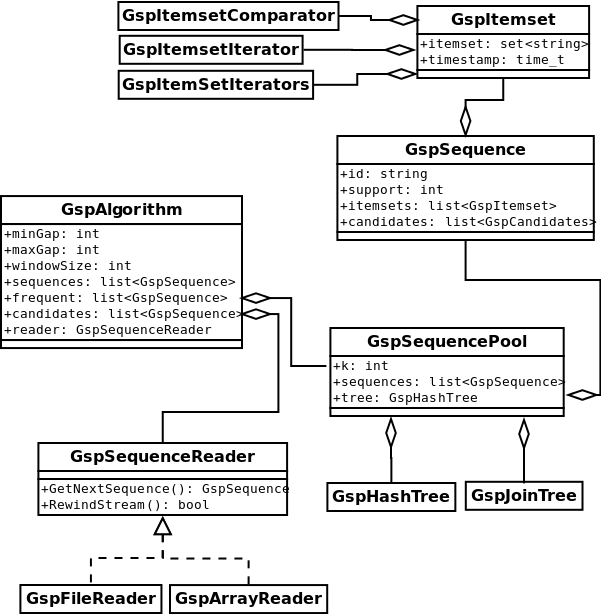
\includegraphics[scale=0.3]{figures/uml-class.png}
\caption{Project class diagram}\label{figure:gsp-class-diagram}
\end{figure}


\section{Input and output data format}

Figure \ref{figure:input-format} depicts an overview of data format used by GSP algorithm implemented for the purpose of the project. 
\begin{figure}[!htb]
\centering
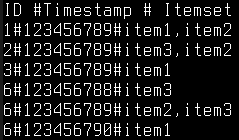
\includegraphics[scale=0.6]{figures/input-format.png}
\caption{Input data format}\label{figure:input-format}
\end{figure}

Data series are in tabular form, where individual columns are separated by a hash symbol. First column of the row corresponds to a unique identifier of the user, second to the timestamp of transaction and the last to a list of comma separated items present in the transaction. 

The output has a form of a simple text file. Each line corresponds to a frequent sequence. Each transaction is printed inside the brackets with the items separated by a space character:
\begin{verbatim}
{ 100 301 }{ 100 }{ 101 317 }{ 307 }
{ 100 307 }{ 100 }{ 101 317 }{ 307 }
\end{verbatim}

\section{User guide}

The resulting program is called \emph{gsp} and is a command-line tool. Some arguments have to be specified for its successful execution:
\begin{verbatim}
./gsp input_file output_file min_sup 
        window_size min_gap max_gap
\end{verbatim}

The arguments have to be specified in given order and their meaning is as following:
\begin{my_itemize}
\item \emph{input\_file} -- the path to the input file.
\item \emph{output\_file} -- the path to the output file for the result sequences. It has to be a writable location. If existing before the operation, the file will be overwritten.
\item \emph{min\_sup} -- the minimum support. A sequence will be considered frequent if its support is larger than the specified value.
\item \emph{window\_size} -- the GSP algorithm sliding windows size.
\item \emph{min\_gap} -- the GSP algorithm minimum gap size.
\item \emph{max\_gap} -- the GSP algorithm maximum gap size.
\end{my_itemize}

\section{Sample data set}

The program was run for a sample data set containing two sequences:
\begin{verbatim}
1#2#1,2,
1#6#1
1#9#1,2
2#2#2
2#9#1,2
2#11#1
\end{verbatim}

The values for the parameters minimal support,window size, minimum and maximum gap were 1, 0, 0, 0 respectively. The resulting frequent sequences were:
\begin{verbatim}
{ 2 }{ 1 }{ 1 }
{ 2 }{ 1 2 }
{ 1 2 }{ 1 }
\end{verbatim}

\section{Results}
The algorithm was run for 3 data sets containing 37, 364 and 3651 data sequences. In each case the the minimum support was set to a value corresponding to 95\% of the overall sequences, the minimum gap was 12 and the maximum gap was 15. Two tests were performed whit different values of the sliding window parameter. In the first case it was set to 0 and in the second it was set to 1.

\begin{table}[!htbp]
\begin{center}
\begin{tabular}{|c|c|c|c|c|}
\hline
\textbf{Support} & \textbf{Window} & \textbf{Time elapsed} & \textbf{Sequences} & \textbf{Length} \\ 
\hline
35/37 & 0 & 0.22 s & 1 & 9 \\
\hline
344/364 & 0 & 14.25 s & 2 & 9 \\
\hline
3450/3651&0 & 164.55 & 3 & 9 \\
\hline
35/37 & 1 & 1.32 s & 3 & 12 \\
\hline
344/364 & 1 & 76.64 s & 3 & 11 \\
\hline
3450/3651 & 1 & 828.22 & 3 & 12 \\
\hline
\end{tabular}
\end{center}
\caption{Results of tests.}  
\label{tab:Res}
\end{table}

As expected, the execution time increases for larger data sets. Also adding the sliding window increases the time needed to perform the operation due to larger number of candidates that meet the minimal support.

%----------------------------------------------------------------------
% SECTION VII: Conclusions
%----------------------------------------------------------------------

\section{Conclusions}

The implemented GSP algorithm proved its correctness by analyzing various small input datasets and comparing the results with straightforwad evaluation. Primarily, the tests with larger input data failed, due to lack of implementing candidates pruning and rather naive method of joining sequences. After implementing candidate pruning as defined in ~\cite{gsp} and using suffix tree for joining sequences the performance increased significantly. Anyhow, even after making these enhancements, the tests involving very large datasets were time consuming. 

Finally, in the analyzed datasets most of the sequences were frequent, it resulted in high memory consumption when processing the data sets. For some program settings the operation could not be finished due to lack of memory. It is caused by huge amounts of candidate sequences generated even for very high minimal support values.

All in all, both the implementation of GSP algorithm and performed tests proved its usefullness and the algorithm procedures defined in ~\cite{gsp} are correct.

\bibliography{mybib}

\end{document}
